%\documentclass[fleqn]{book}
\documentclass[11pt]{amsbook}

\usepackage[turkish]{babel}

\usepackage{../Ceyhun}	% ------------------------
\usepackage{../amsTurkish}


\begin{document}
% ++++++++++++++++++++++++++++++++++++++
\hPage{194}
% ++++++++++++++++++++++++++++++++++++++
\par
{\itshape Durum 1 :} 

$d_0$, $Ç$ nin dışına çizilemediğine göre $d_0$, $Ç$ ye en az üç yolla bağlıdır (\ref{fig}a). Bu da ,
$Ç(d,a)$ içinde, $\Theta_1$ çizgesi ile kökteş bir altçizgenin varolması demektir. \\

\par
{\itshape Durum 2 :} 

$d_0$, $Ç$ nin dışına çizilemediğine göre ve $Ç$ ye en az üç yolla bağlı olmadığına göre, $d_0$, $Ç$ ye iki yolla 
bağlıdır. (bir yolla bağlı olsaydı $Ç$ nin üzerinde, $d_1$ ve $d_2$ nin dışına çizilebilirdi). Ayrıca $Ç$ nin üzerinde, 
$d_1$ ve $d_2$ nin dışında, \ref{fig}b de gösterildiği gibi
\begin{figure}[htb]
	\centering
	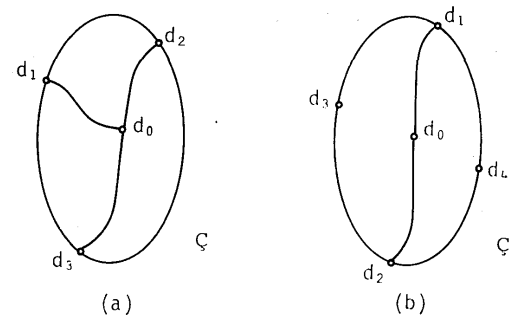
\includegraphics[width=0.65\textwidth]{images/ceyhun-194-fig.png}
	\caption{Teorem 4.1.8 in tanıtı.}
	\label{fig}
\end{figure}
en az iki düğüm daha vardır. Bu da, $Ç(d,a)$ nın içinde $\Theta_2$çizgesi ile kökteş bir çizgenin varolması demektir.
\end{document}